% Автор разбора: Антон Ахи

\begin{frame}
  \frametitle{Задача <<Бендер>>}
  \begin{center}
    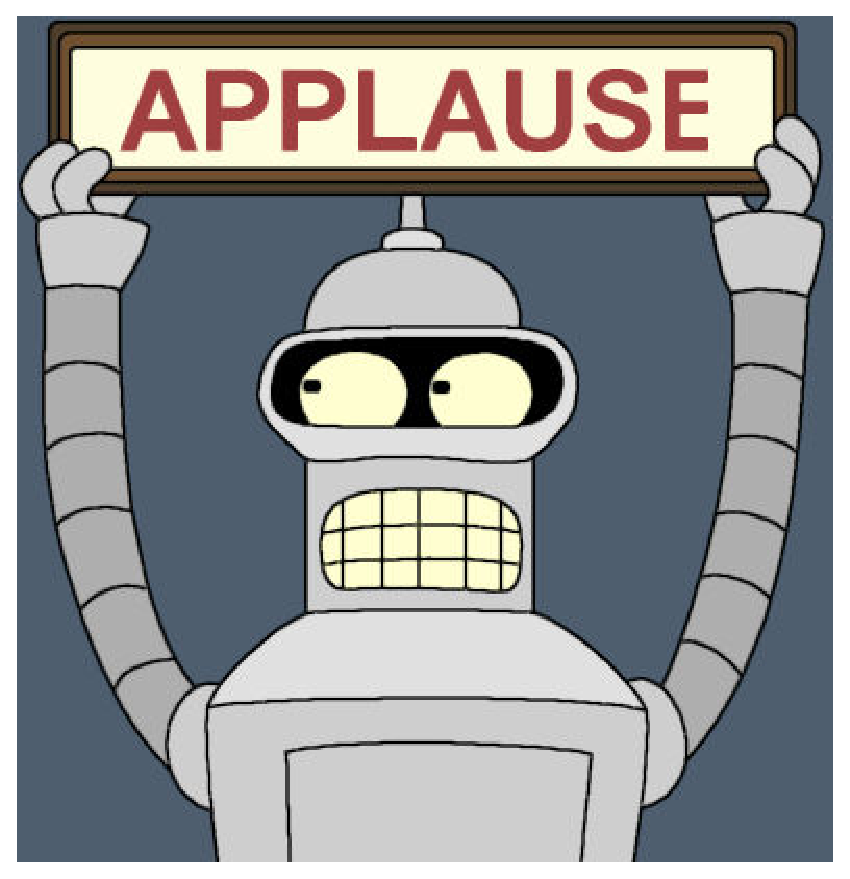
\includegraphics[height=9cm]{bender.eps}
  \end{center}
\end{frame}

\begin{frame}
  \frametitle{Над задачей работали}
  \begin{itemize}
    \item Идея задачи: Антон Банных
    \item Текст условия: Антон Ахи
    \item Тесты, проверяющая программа и др.: Владимир Ульянцев
    \item Решения: Антон Банных, Михаил Майоров 
    \item Текст разбора: Антон Ахи
  \end{itemize}
\end{frame}

\begin{frame}
  \frametitle{Формулировка задачи}
  \begin{itemize}
    \item Робот Бендер строит последовательность $x_i$ из $n$ элементов
    \item $x_1 = c$; $x_i = a \cdot x_{i - 1} + b$ для $i > 1$
    \item На $i$-ом шаге меняются местами стаканчики на позициях $(x_i \mod k) + 1$ и
    		$(x_{i + 1} \mod k) + 1$
    \item Найти $a$, $b$ и $c$ такие, чтобы шарик под стаканчиком на позиции $r$ после $n$ дейтсвий
    		оказался под стаканчиком на позиции $l$  
  \end{itemize}
\end{frame}

\begin{frame}
  \frametitle{Идея решения}
  \begin{itemize}
    \item Так как $k$ невелико и важно лишь значение $x_i \mod k$,
    		то можно перебрать все возможные $a$, $b$ и $c$ от $0$ до $k - 1$ и проверить их  
    \item Проверку осуществлять за $O(n)$, совершая все обмены
    \item Если ответ найдет, вывести его, иначе вывести <<\texttt{Impossible}>>
  \end{itemize}
\end{frame}

\begin{frame}
  \frametitle{Итого}
  \begin{itemize}
    \item Решение совершает $O(n \cdot k^3)$ операций 
    \item Вопросы?
  \end{itemize}
\end{frame}